\documentclass[11pt]{toptesi}
%%%%%%%%%%%%%%%%%%%%%%%%%%%%%%%%%%%%%%%%%%%%%%%%%%%%%%%%%%%%%%%

% INCLUSIONE PACCHETTI
\usepackage[utf8]{inputenc} %utf8
\usepackage[italian]{babel}
%\usepackage[T1]{fontenc}
\usepackage{blindtext}
\usepackage{graphicx,wrapfig}
\usepackage{booktabs}
\usepackage{lmodern}
\usepackage{varioref}
\usepackage{url}
\usepackage{array}
\usepackage{paralist}{\obeyspaces\global\let =\space}
\usepackage{verbatim} 
\usepackage{subfig}	%per figure affiancate. Sostituisce subfigure
\usepackage{tabularx}
\usepackage{amsmath}
\usepackage{amsfonts}
\usepackage{float}
\usepackage{amssymb}
\usepackage{multicol}
\usepackage{multirow}
\usepackage{listings}
\usepackage[pass]{geometry}
\usepackage[figuresright]{rotating}
\usepackage{algorithm}
\usepackage{algorithmic}
\usepackage{amsmath}
\usepackage[babel]{csquotes}
\usepackage{hyperref}
\usepackage[backend=bibtex]{biblatex}

\usepackage[skip=0.01pt]{caption}


%%%%%%%%%%%%%%%%%%%%%%%%%%%%%%%%%%%%%%%%%%%%%%%%%%%%%%%%%%%%%%%

% CONFIGURAZIONE LINK E RIFERIMENTI
\hypersetup{
    pdfpagemode={UseOutlines},
    bookmarksopen,
    pdfstartview={FitH},
    colorlinks,
    linkcolor={black}, %COLORE DEI RIFERIMENTI AL TESTO
    citecolor={black}, %COLORE DEI RIFERIMENTI ALLE CITAZIONI
    urlcolor={blue} %COLORI DEGLI URL
}

%%%%%%%%%%%%%%%%%%%%%%%%%%%%%%%%%%%%%%%%%%%%%%%%%%%%%%%%%%%%%%%

% CONFIGURAZIONE LISTATI/CODICE - CANCELLARE SE NON NECESSARIO
% JAVA - BIANCO E NERO
\lstset{%
	captionpos=b,
	language=Java,
	basicstyle =\small\ttfamily,
	keywordstyle=\color{black}\bfseries,
	breaklines=true,
	breakatwhitespace=true,
	frame=lines,
	numbers=left,
	numberstyle=\footnotesize,
}

%%%%%%%%%%%%%%%%%%%%%%%%%%%%%%%%%%%%%%%%%%%%%%%%%%%%%%%%%%%%%%%

% FRENCHSPACING VA _SEMPRE_ ABILITATO PER DOCUMENTI IN ITALIANO
\frenchspacing

%%%%%%%%%%%%%%%%%%%%%%%%%%%%%%%%%%%%%%%%%%%%%%%%%%%%%%%%%%%%%%%

%DEFINIZIONE SEZIONI IN NUMERAZIONE ROMANA
%ELENCO DEI LISTATI/CODICI
\makeatletter
\newcommand\listofcodes{%
 \iffrontmatter\else\frontmattertrue\fi
 \if@openright\cleardoublepage\else\clearpage\fi
 % change the meaning of \chapter in a group
 \begingroup\def\chapter##1{\@schapter}
 \phantomsection % for the hyperlink
 \lstlistoflistings 
 \endgroup
} 
\makeatother

%%%%%%%%%%%%%%%%%%%%%%%%%%%%%%%%%%%%%%%%%%%%%%%%%%%%%%%%%%%%%%%

% INFORMAZIONI PDF - PERSONALIZZARE
\pdfinfo{%
  /Title    (Codifica video intelligente)
  /Author   (Matteo Tintori)
  /Subject  (@)
  /Keywords ( )
}
%%%%%%%%%%%%%%%%%%%%%%%%%%%%%%%%%%%%%%%%%%%%%%%%%%%%%%%%%%%%%%%


% FRONTESPIZIO - PERSONALIZZARE
% ELIMINATE LE VOCI CHE NON VI SERVONO

% UNIVERSITA - NOME
\ateneo{Università degli Studi di Firenze}

% FACOLTA - DICITURA - CANCELLARE O DECOMMENTARE
\FacoltaDi{Scuola di}
% FACOLTA - NOME
\facolta{ Ingegneria\\Dipartimento di Ingegneria dell'Informazione}

% CORSO DI LAUREA - DICITURA (MANTENERE LO SPAZIO) - CANCELLARE O DECOMMENTARE
\CorsoDiLaureaIn{Laurea Triennale in }
% CORSO DI LAUREA - NOME
\corsodilaurea{Ingegneria Informatica}

% TIPOLOGIA TESI
\TesiDiLaurea{Tesi di Laurea Triennale}

% TITOLO
\titolo{Codifica video intelligente con l'uso di Faster-RCCN e CODEC H.265 esteso con selezione basata su RoI}

% SOTTOTITOLO
%\sottotitolo{}

% RELATORE/I - DICITURA - CANCELLARE SE UN SOLO RELATORE
%\AdvisorName{Relatori}
% RELATORE - PROF. NOME E COGNOME
\relatore{Chiar.mo Prof.Bertini Marco}

% CANDIDATO - DICITURA (MANTENERE I DUE PUNTI) - CANCELLARE O DECOMMENTARE
%\CandidateName{Candidate:}

% CANDIDATO - NOME E COGNOME
\candidato{Matteo Tintori}


% LOGO UNIVERSITA
\logosede{images/logo}

% DATA - MESE ANNO
\sedutadilaurea{Anno Accademico 2019-2020}
% LISTA DEI CAPITOLI DA INCLUDERE - PERSONALIZZARE
%\includeonly{%
%introduzione%
%}
%%%%%%%%%%%%%%%%%%%%%%%%%%%%%%%%%%%%%%%%%%%%%%%%%%%%%%%%%%%%%%%
\bibliography{bibliography}
\begin{document}
\frontespizio
%%%%%%%%%%%%%%%%%%%%%%%%%%%%%%%%%%%%%%%%%%%%%%%%%%%%%%%%%%%%%%%

%INTERLINEA - DEFAULT 1 - NON ESAGERATE, NON SUPERATE MAI 1.3 ;)
\interlinea{1.1}

%%%%%%%%%%%%%%%%%%%%%%%%%%%%%%%%%%%%%%%%%%%%%%%%%%%%%%%%%%%%%%%

\frontmatter

% DEDICA - PERSONALIZZARE
% VSPACE - PROPORZIONE USATA PER CENTRATURA VERTICALE DEL TESTO
% FLUSHRIGHT - ALLINEAMENTO ORIZZONTALE A DESTRA
\vspace*{\stretch{1}}
\begin{flushright}
\noindent
Alla mia famiglia che ha garantito per ogni bisogno in tutto il percorso di studi.\\
\vspace{1cm}
Ai compagni,alla donna e agli amici che mi hanno accompagnato e in particolare a quelli che mi hanno sostenuto fino agli ultimi esami. \\
\vspace{1cm}
Al \textit{Prof. Bertini Marco} per la disponibilità e professionalità nel fornire ogni tipo di materiale e aiuto.
\end{flushright}
\vspace*{\stretch{6}}
\cleardoublepage


% CITAZIONE - PERSONALIZZARE
% VSPACE - PROPORZIONE USATA PER CENTRATURA VERTICALE DEL TESTO
% FLUSHRIGHT - ALLINEAMENTO ORIZZONTALE A DESTRA
\vspace*{\stretch{1}}
\begin{flushright}
\noindent
La pazienza è amara, ma dolce è il suo frutto. \\
\textit{(Jean-Jacques Rousseau)}
\end{flushright}
\vspace*{\stretch{6}}
\cleardoublepage

%%%%%%%%%%%%%%%%%%%%%%%%%%%%%%%%%%%%%%%%%%%%%%%%%%%%%%%%%%%%%%%
% RINGRAZIAMENTI - PERSONALIZZARE
%\ringraziamenti


%%%%%%%%%%%%%%%%%%%%%%%%%%%%%%%%%%%%%%%%%%%%%%%%%%%%%%%%%%%%%%%

% INDICI - ELIMINARE GLI INDICI NON NECESSARI

% INDICE GENERALE
%\tableofcontents

% INDICE DELLE FIGURE
%\listoffigures

%% INDICE DELLE TABELLE
%%\listoftables

%% INDICE DEI CODICI
%%\listofcodes

%%%%%%%%%%%%%%%%%%%%%%%%%%%%%%%%%%%%%%%%%%%%%%%%%%%%%%%%%%%%%%%

\mainmatter

% INCLUSIONE FILE CAPITOLI - PERSONALIZZARE - TENERE COERENTE CON LISTA IN ALTO
\chapter{Introduzione}
\label{chap:intro}
%Introduzione su cosa ho fatto

\section{Intento}
\label{sec:intento}
%Identifica il prodotto, includendo versione di revisione e/o rilascio. 

L'obbiettivo di questo elaborato è la realizzazione di un Codec a partire da formato \textbf{H.265} destinato a video di calcio HD, che performi una compressione altrettanto efficiente ma variabile sulla base del contenuto interessante di ogni singolo frame.
In particolare, si vuole codificare una partita di calcio utilizzando reti neurali convoluzionali per il riconoscimento e la conseguente segmentazione dei giocatori sul campo, e quando possibile, della palla. 
Le posizioni delle suddette entità sono le regioni di interesse che saranno lasciate senza perdita di qualità, mentre sulle altre zone verrà applicato un filtro che fornirà una compressione migliore "sacrificando" le alte frequenze e quindi una piccola parte di informazione non interessante. Viene poi effettuato un confronto tra il video originale e quello codificato come indice di efficienza, utilizzando metriche di qualità oggettiva. Infine, come indice di miglior codifica, viene effettuato un confronto tra i risultati di questo prodotto e un altro prodotto basato su Codec x264 e salienza, intesa come punto centrale dove l'osservatore è abituato a guardare spontaneamente, e se ne deduce il migliore in termini di dimensioni del prodotto compresso risultante.


\section{Ambito del progetto}
\label{sec:projscope}
%Breve descrizioni del software , includendo benefici, obiettivi e goals.
Il software si colloca nel campo della computer vision e si vuole affermare come Codec \textbf{H.265} che punta a comprimere più informazioni delle librerie già usate, valido particolarmente nei casi in cui ci sia una limitazione di spazio nel device in cui si scarica/guarda il video o nel caso si debba risparmiare per motivi economici sulla quantità di dati scaricati (ad esempio una soglia di (G)byte massima fissata dal gestore telefonico). 
Il Codec non si propone come versione superiore delle implementazioni già esistenti di \textbf{H.265} ma piuttosto come alternativa semantica.
\\
\chapter{Strumentazione}
\label{chap:tools}

\section{Piattaforma di sviluppo}
\label{sec:platform}
La workstation usata per lo sviluppo del software è un server Linux con 2 schede video NVIDIA Titan X ed è collegata alla rete con IP pubblico all'indirizzo solaris.micc.unifi.it ed accedibile con utente mtintori. 
La modalità di lavoro perseguita è remota utilizzando remote desktop da PC Windows e PC Mac in seguito.
L'IDE utilizzato per lo sviluppo è Pycharm con versione di Python 3.6.

\section{Miniconda}
Miniconda è un gestore di pacchetti ed environment-manager. E' una versione di installazione minimale di Anaconda, comprende l'interprete Python e permette di utilizzare un'IDE alternativo a Spider, usato con Anaconda, inoltre non vengono installati gli oltre 250 pacchetti che sono compresi nell'installazione di Anaconda lasciando la libertà allo sviluppatore su quali pacchetti installare.
\label{sec:miniconda}
\subsection*{Ambienti Miniconda}
Utilizzeremo il termine Conda, istruzione fondamentale Miniconda, per riferirsi al sunnominato manager.
Per la realizzazione del Codec si è resa necessaria la creazione di due ambienti Conda: è stata effettuata una simile scelta per possibilità di debug anche in assenza di rete su una workstation personale che non possiede una GPU. 
\begin{itemize}
\item \emph{tf\_cpu} : ambiente più lento, ma utilizzabile anche da una workstation non avente GPU
\item \emph{tf\_gpu} : ambiente più veloce, ma utilizzabile solo da una workstation con una GPU con ampia memoria adatta al training di reti neurali
\end{itemize}
\section{Schema del sistema}
\begin{figure}
   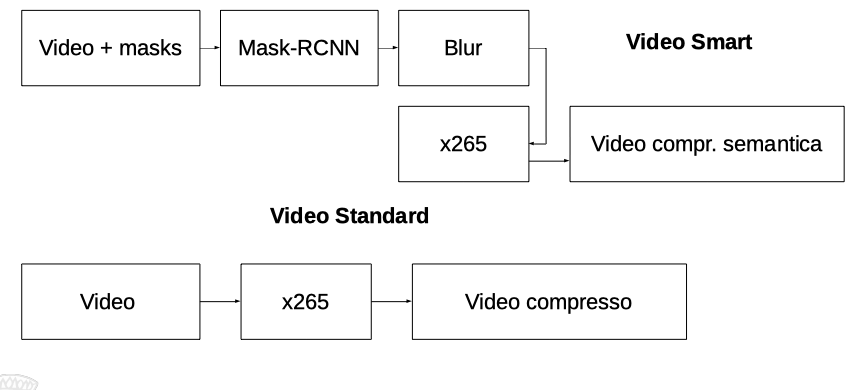
\includegraphics[width=\linewidth]{images/schema.png}
   \caption{}
   \label{fig:c}
\end{figure}
\section{CODEC di partenza}
\label{sec:codec_base}
%Descrivere il codec
La scelta del codec da utilizzare era contesa tra gli standard candidabili \textbf{H.264}, \textbf{H.265}, mentre gli altri due standard ottimali \textbf{VP9} e \textbf{AV1} non sono stati volontariamente presi in considerazione come assunto iniziale, nonostante le performance del secondo qualche volta superiore a \textbf{H.265} implementato dall'encoder \textbf{x265}.\textsuperscript{\ref{fig:c}} (si noti che \textbf{VP9} invece è visibilmente inferiore agli altri,come si nota pur dalle info \textbf{libvpx}\textsuperscript{\cite{libvpx}} che lo implementa).
\begin{figure}
   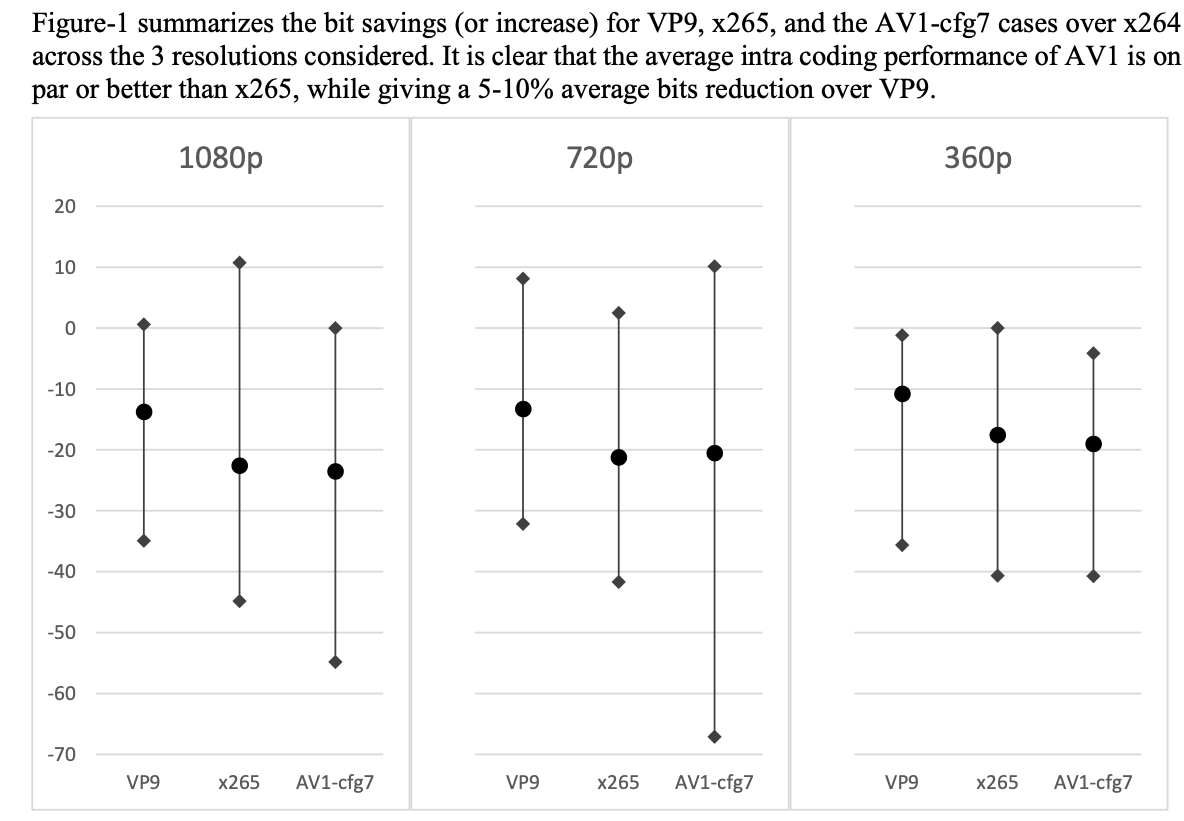
\includegraphics[width=\linewidth]{images/x265vsAv1.png}
   \caption{Risparmio in bits (segni: - risparmio, + incremento)}
   \label{fig:c}
\end{figure}
\\Sappiamo anche che \textbf{x264} implementa lo standard precedente; è quindi sicuramente più scarso. Lo standard dalla quale siamo partiti per una codifica efficiente è allora \textbf{H.265} usando \textbf{hevc\_nvenc} \textsuperscript{\ref{sec:nvenc}}, ed abbiamo optato per una codifica progressiva frame per frame. Il nostro encoder prevede una quantizzazione "doppia", poiché prima di scrivere ogni frame vengono selezionate le regioni non interessanti e ne vengono tagliate fuori le HF\footnote{Alte frequenze}; ciò verrà spiegato in seguito. Quello che invece fa il Codec di partenza che abbiamo scelto è una quantizzazione secondo lo standard, che viene effettuata manovrando il parametro \emph{QP} cui valore rappresenta la sua intensità, ovvero quanta informazione (sempre HF) viene scartata.
\subsection*{CRF}
Il Costant Rate Factor\textsuperscript{\cite{CRF_vs_QP}}  è un fattore che influenza la quantizzazione in modo più sofisticato del parametro a basso livello \emph{QP} previsto dallo standard H.265. Più alto il CRF, più i campioni (pixel o blocchi di pixel) vengono quantizzati in maniera maggiore; questo valore resta fisso per l'intera codifica del video scelto, mentre il valore del parametro \emph{QP} varia a seconda di quanto si debba quantizzare in ogni frame per mantenere una qualità costante.
Nel nostro caso, utilizzando \textbf{nvenc} non sarà presente il parametro \emph{crf} ma si deve utilizzare il parametro equivalente \emph{cq} di questa libreria a cui sarà dato un valore che garantirà una compressione visivamente lossless, ovvero con perdita di qualità trascurabile all'occhio umano; essenzialmente questo valore per \textbf{h264\_nvenc} è circa 19 per cui, preso atto che il valore di default di \textbf{x264} è 23 e corrisponde a circa 28 di \textbf{x265}, non sbaglieremo nel dire che 19 è sicuramente visually lossless anche per \textbf{hevc\_nvenc}.
\section{FFMPEG}
\label{sec:coding_library}
%Descrivere il codec
Utilizzando la libreria \textbf{FFMPEG} è stato possibile scegliere diversi parametri oltre al Codec \textbf{hecv\_nvenc}. 
Le modalità tipiche di codifica sono 3: \footnote{vedi rate control modes: https://trac.ffmpeg.org/wiki/Encode/H.265} 
\begin{enumerate}
\item bitrate scelto in 1 passo (sconsigliato)
\item bitrate scelto in 2 passi
\item CRF (fattore di qualità costante)
\end{enumerate}
Dal momento che non è nostro interesse il raggiungimento di una dimensione file particolare, la scelta è caduta sulla terza opzione, che è stata spiegata nella sottosezione precedente.
Gli altri parametri che abbiamo utilizzato per la codifica sono i seguenti:
\begin{itemize}
\item \textbf{-cq}: fattore di qualità che mantiene la suddetta costante in ogni frame manovrando il parametro che definisce la quantizzazione \emph{QP}
\item \textbf{-qmin} : fattore minimo di qualità che \textbf{cq} può assumere
\item \textbf{-qmax} : fattore massimo di qualità che \textbf{cq} può assumere
\item \textbf{-b:v} : posto a 0 per causa di un bug nella libreria, che se non venisse settato inibisce il funzionamento di cq
\item \textbf{-rc} : rate control, sovrascrive la velocità di compressione ("preset",più basso il preset più alta la qualità) e deve essere settato insieme a \textbf{\emph{-b:v}} per una qualità costante
\item \textbf{-r} : frame rate, ovvero quanti frame vengono campionati nell'unità di tempo
\end{itemize}
%Descrivere l'ambiente in cui opererà il software, includendo piattaforme hardware, altri sistemi operativi con relativa versione, altre componenti software che utilizza questo prodotto

\section{Mask-RCNN}
\label{sec:Mask-RCNN_desc}
Mask-RCNN è un'implementazione di una rete neurale Faster-RCNN da parte del framework tensorflow di Google. Si differenzia dalle Faster-RCNN per l'introduzione del RoI Align, più preciso rispetto al RoI Pooling precedente. Facciamo un piccolo riepilogo per maggiore chiarezza.
\subsection*{Riepilogo - Dalle CNN alle Faster-RCNN}
Le reti neurali convoluzionali \textbf{(CNN)} sono state introdotte nel campo dell' IA per vari scopi e più precisamente nella computer vision sono utili per il riconoscimento di qualsiasi entità o pattern all'interno di un immagine. Le potenzialità e i limiti sono elencati di seguito:
\begin{enumerate}
\item Usano una funzione softmax per classificazione multi-classe e sigmoid per classificazione binaria
\item Usata per image classification e object detection
\item Rileva solo un oggetto alla volta senza sovrapposizioni
\end{enumerate}
Successivamente si sono affermate le CNN basate su regioni \textbf{(RCNN)}, che forniscono il miglioramento di riconoscere più oggetti diversi nella stessa immagine e identificarli all'interno di un rettangolo. Questo è possibile con il seguente procedimento:
\begin{enumerate}
\item Generazione di regioni propositive con R-CNN per mezzo dell'algoritmo \emph{Selective Search} unito con \emph{Exhaustive Search}
\item Fusione di regioni propositive simili e \emph{Feature extraction} con CNN per ogni regione propositiva
\item Algoritmo \emph{Support vector machine} per la feature estratta per la verifica dell'effettiva presenza dell'oggetto 
\item Algoritmo \emph{Non-Max suppression} per lo scarto di regioni con basso punteggio in \emph{Intersection over Union}.
\end{enumerate}
Per ottenere un altro significativo miglioramento siamo arrivati alle reti \textbf{Fast-RCNN}, che offrono i seguenti vantaggi:
\begin{enumerate}
\item Unica rete neurale (deep ConvNet) che sostituisce quelle migliaia di R-CNN sulle singole regioni
\item Unico modello per la feature extraction, la classificazione e le bounding boxes
\item Introduzione delle Region of Interest (RoI) e del RoI Pooling
\end{enumerate}
Infine, si è voluto perfezionare l'arte del riconoscimento e identificazione delle forme di ogni entità con le reti \textbf{Faster-RCNN}, che permettono di:
\begin{enumerate}
\item 3-D object detection
\item Part-based detection
\item Instance segmentation
\item Image captioning
\end{enumerate}




\chapter{Sistema di segmentazione oggetti}
\label{chap:preparation}
In questo capitolo, per iniziare, si vuole distinguere la differenza tra un training di una rete blackbox e un fine tuning di una rete preaddestrata.\\
Essendo \textbf{Mask-RCNN} una rete preaddestrata per circa 60 classi, si parlerà innanzitutto di un fine tuning e non di un allenamento di una rete partendo da zero esperienza(blackbox).\\
La cosa che distingue il nostro agire in questo caso è che faremo un fine tuning, non sulle circa 60 classi sulla quale è stata preaddestrata la rete, ma solamente su 2 classi che rappresenteranno i giocatori e la palla all'interno del campo di calcio.
\newpage
\section{Strutturazione Fine-Tuning}
Come premessa, bisogna dichiarare il fatto che per un buon fine tuning serve scegliere un software di labeling che fornisce le annotazioni in un certo formato, solitamente XML.
Nel nostro caso, siccome sappiamo che PASCALVOC XML viene usato quando c'è da fare object detection mentre noi cerchiamo di fare instance segmentation, abbiamo usato un software chiamato \textbf{labelme} che produce annotazioni con estensione JSON in modo da prelevare facilmente i dati dei poligoni racchiusi nei files.
Lo strumento \textbf{labelme} viene utilizzato per tracciare poligoni intorno ai giocatori nei frames, cioè le immagini singole di un video che è stato frammentato con uno strumento come ad esempio \textbf{Avidemux}. \\
Nel software \textbf{labelme} quando viene scelto un tracciamento della curva \emph{poligono}, questi poligoni devono essere tracciati come linea spezzata chiusa con un numero di punti adatto a circondare con la minima tolleranza possibile la forma di un giocatore, e nel caso della scelta sul software \textbf{labelme} della curva \emph{cerchio}, esso andrà a circondare la palla.
Chiaramente, un giocatore potrà essere all'interno del campo in diverse posizioni, ad esempio in piedi fermo, in piedi in corsa oppure a terra come dopo una parata o una scivolata; tutti questi casi devono essere circondati da punti che formano un poligono per far sì che la rete \textbf{MaskRCNN} abbia un allenamento soddisfacente.\\
Una volta salvato il frame modificato con i poligoni, il software \textbf{labelme} genererà un file JSON con all'interno i dati del nome dell'immagine, la sua altezza e larghezza, il numero e i punti dei poligoni in modo da essere letti successivamente da codice.
L'operazione di contornamento dei giocatori e della palla con i poligoni di punti, si chiama \textbf{labeling}, e si può effettuare un labeling anche massivo specificando all'apertura del software \textbf{labelme}  una directory dove sono presenti tutti i frames del video obbiettivo e in contempo una directory vuota dove produrre in massa i file JSON delle loro annotazioni; ogni file di annotazione viene prodotto non appena il labeling di un immagine viene ultimato e quindi l'immagine viene salvata.
%%%%%%%%%%%%%%%%%%%%%%%%%%%%%%%%%%%%%%%%%%%%%%%%%%%%
%\appendix
% INCLUSIONE APPENDICI - - PERSONALIZZARE - TENERE COERENTE CON LISTA IN ALTO

%%%%%%%%%%%%%%%%%%%%%%%%%%%%%%%%%%%%%%%%%%%%%%%%%%%%%%%%%%%%%%%
\nocite{*}
\addcontentsline{toc}{chapter}{Bibliography}
\printbibliography
\end{document}